% rubber: set program xelatex
\documentclass[18pt,mathserif]{beamer}

%{{{ Settings
\usetheme[english, titlepage0]{KIT}

%{{{ Packages
\usepackage{tikz}
%\usepackage{xltxtra}
\usepackage{csquotes}
\usepackage{caption}
\usepackage{hyperref}
\usepackage[framemethod=tikz]{mdframed}
%}}}
%{{{ Fonts and colors
%\setsansfont[Mapping=tex-text,
%             BoldFont={* Semibold}]{Source Sans Pro}
%\setmonofont[UprightFeatures={LetterSpace=-0.5}]{Inconsolata}

% TomorrowTheme: https://github.com/chriskempson/tomorrow-theme/blob/master/vim/colors/Tomorrow.vim
\definecolor{syntax-comment}{HTML}{8e908c}
\definecolor{syntax-keyword}{HTML}{8959a8}
\definecolor{syntax-number}{HTML}{eab700}
\definecolor{syntax-green}{HTML}{718c00}
\definecolor{syntax-red}{HTML}{c82829}

\setbeamercolor{section in toc}{fg=black!80}
%}}}
%{{{ TikZ styles
\usetikzlibrary{arrows, backgrounds, calc, trees, shapes, snakes}

\tikzset{
  commit/.style={
    circle, draw, color=black!75, fill=syntax-keyword!75,
    line width=1pt, minimum height=12pt
  },
  connection/.style={
    draw, ->, >=stealth, color=black!75, line width=.75pt
  }
}

\pgfdeclareimage[width=.36cm]{butthurt}{images/butthurt}

\newcommand\score[2]{
  \pgfmathsetmacro\pgfxa{#1+1}
  \begin{tikzpicture}[baseline=-3pt]
    \foreach \i in {1,...,#2} {
      \pgfmathparse{(\i<=#1?"1.0":"0.3")}
      \edef\starcolor{\pgfmathresult}
      \node[name=butthurt\i, opacity=\starcolor, inner sep=0pt] at (\i*3ex,0) {\pgfuseimage{butthurt}};
    }
  \end{tikzpicture}
}

\makeatletter
\tikzset{
  circle split part fill/.style  args={#1,#2}{%
    alias=tmp@name, % Jake's idea !!
    postaction={%
      insert path={
        \pgfextra{%
          \pgfpointdiff{\pgfpointanchor{\pgf@node@name}{center}}%
                       {\pgfpointanchor{\pgf@node@name}{east}}%
          \pgfmathsetmacro\insiderad{\pgf@x}
          \fill[#1] (\pgf@node@name.base) ([xshift=-\pgflinewidth]\pgf@node@name.east) arc
                            (0:180:\insiderad-\pgflinewidth)--cycle;
          \fill[#2] (\pgf@node@name.base) ([xshift=\pgflinewidth]\pgf@node@name.west)  arc
                            (180:360:\insiderad-\pgflinewidth)--cycle;
        }
      }
    }
  }
}
\makeatother
%}}}
%{{{ Environments
\makeatletter
\newenvironment{shell}[1][\linewidth]
  {\begin{mdframed}[
  skipabove=\topsep,
  skipbelow=\topsep,
  font=\ttfamily,
  linecolor=black!9,
  backgroundcolor=black!9,
  innertopmargin=6pt,
  innerbottommargin=6pt,
  innerleftmargin=6pt,
  innerrightmargin=6pt,
  userdefinedwidth=#1]}
  {\end{mdframed}}
\makeatother
%}}}
%{{{ Meta
\title{Version Control with Git}
\author{Eileen K\"uhn, David Kunz, Sarah M\"uller, Robin Roth}
\subtitle{Eileen K\"uhn, David Kunz, Sarah M\"uller, Robin Roth}
\institute{KSETA Doktorandenworkshop, 23.07.2014}
\date{Jul.~23\textsuperscript{rd} 2014}

\graphicspath{{../../common/}}

% TODO: schoeneres Logo
\TitleImage[width=4cm]{images/octocat.png}
%}}}

%}}}

\begin{document}
\maketitle

\section{Motivation}

\begin{frame}{Plead guilty!}
  It's easy to copy digital content, so why not re-create it over and over
  again?

  \begin{columns}[onlytextwidth]
    \visible<2->{
      \column{0.5\textwidth}
        \begin{figure}
          \centering
          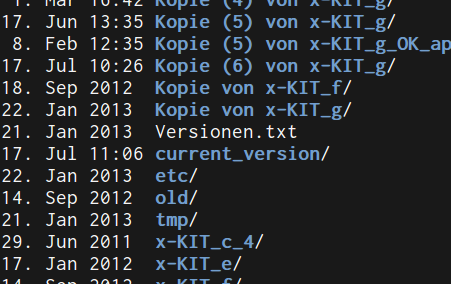
\includegraphics[width=4.5cm]{images/mrcs.png}
          \caption*{\enquote{One of these folders \emph{must} contain the latest
          version \ldots}}
        \end{figure}
    }

    \visible<3->{
      \column{0.5\textwidth}
        \begin{figure}
          \centering
          
\includegraphics[width=4.5cm]{images/reports.png}
          \caption*{\enquote{Here is the latest version of the
          proposal/paper/report.} --- \enquote{Thanks.}}
        \end{figure}
    }
  \end{columns}
\end{frame}
\begin{frame}{Obvious disadvantages}
  \begin{itemize}
    \item No meta data about \emph{what} was changed \emph{when} by
      \emph{whom}
    \item You lose track of what's going on
    \item You cannot easily roll-back to a working state
    \item Poor solution for collaboration
  \end{itemize}
\end{frame}
\begin{frame}{Version control}
	\begin{itemize}
		\item \emph{Track} files
		\item Record (\emph{commit}) changes
		\item Share changes with others
		\item Roll-back to an earlier state
		\item Implicit backup

	\end{itemize}
\end{frame}

\begin{frame}{Why Git?}
  \begin{columns}[T,onlytextwidth]
    \column{0.7\textwidth}
        \begin{itemize}
          \item De-facto standard for open source software
          \item Probably the fastest version control system out there
          \item GitHub: web based collaboration platform
					\item Works well both with central and distributed repositories
					\item Easy to learn
        \end{itemize}
    \column{0.3\textwidth}
      \centering
      
\includegraphics[width=4.0cm]{images/octocat.png}
  \end{columns}
\end{frame}

\section{Hands-on introduction}

\begin{frame}{}
  \begin{center}
    \huge\bfseries
    \textcolor{KITblack}{Git Basics}
  \end{center}
\end{frame}

\begin{frame}{Single User Workflow}
  \begin{enumerate}
    \item Create a repository and a branch ``master''
      \begin{shell}
        \$ git init
      \end{shell}
    \item Create a commit
      \begin{enumerate}
        \item Add something to the commit
          \begin{shell}
            \$ git add README.txt
          \end{shell}
        \item Perform the commit
          \begin{shell}
            \$ git commit -m "Added a README file"
          \end{shell}
      \end{enumerate}
  \end{enumerate}
	\begin{center}
	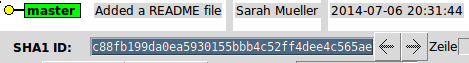
\includegraphics[width=.8\linewidth]{pics/init0.png}
	\end{center}
\end{frame}

% Live Demo 1

\begin{frame}{Commits}
  Everytime you make a change, you create a \alert{commit} containing:
  \begin{itemize}
    \item added/removed lines in files
    \item a comment summarizing what was changed
    \item an author
    \item a date
    \item a checksum (SHA-hash) to identify the commit
    \item a reference to the previous state of your files (parent(s))
  \end{itemize}
\end{frame}

% \begin{frame}{Commit Graphs}


%   \begin{itemize}
%     \item The first commit does not have a parent. It creates a \alert{repository}.
%     \item Multiple co mmits can have the same parent (e.g. when coworkers work on the same code).
%     \item Commits can have multiple parents if the two diverging changes are merged.
%     \item Commits can have \alert{labels}. Labels can be e.g. branch names version tags.
%   \end{itemize}
% \end{frame}


\begin{frame}[t]{Single User Workflow}
  \begin{enumerate}
    \item<alert@1> Change something, and inspect the difference to the last commit
      \begin{shell}
        \$ vi README.txt\\
        \$ git diff\\
      \end{shell}
    \item Create a commit (as before)
      \begin{enumerate}
        \item<alert@2> Add some changes to the commit
          \begin{shell}
            \$ git add README.txt
          \end{shell}
        \item<alert@3> Perform the commit
          \begin{shell}
            \$ git commit -m "Added project description"
          \end{shell}
      \end{enumerate}
  \end{enumerate}
  \begin{overprint}
		\includegraphics<1>[width=.8\linewidth]{pics/commit0.png}
		\includegraphics<2>[width=.8\linewidth]{pics/commit1.png}
		\includegraphics<3>[width=.8\linewidth]{pics/commit2.png}
    \end{overprint}
\end{frame}

\begin{frame}{How to commit} 
  \begin{itemize}
    \item Small logical units
    \item Several times an hour 
			%TODO: add pic
    \item Check the status before committing
    \item Write descriptive commit messages and keep 50/72 limits
		\item[$\Rightarrow$] Allows you to retrace your steps
   \end{itemize}
 \end{frame}

\begin{frame}{Branching}
  \begin{itemize}
		\item Keep master branch free from ``questionable'' code
			\begin{itemize}
				\item Working on independent features at the same time
				\item Trying incompatible changes
				\item Quick and dirty work without changing the master branch
			\end{itemize}
		\item Cheap, instant and easy
		\item Create and destroy often
		\item Integral part of a typical Git workflow
  \end{itemize}
\end{frame}

\begin{frame}[t]{Branching}
    \begin{itemize}
        \item Create two branches from master
            \begin{shell}
                \alert<1>{\$ git checkout master}\\
                \alert<2>{\$ git checkout -b featureA}\\
                \alert<2>{\$ ...change \& commit something}\\
                \alert<3>{\$ git checkout master}\\
                \alert<4>{\$ git checkout -b featureB}\\
                \alert<5>{\$ ...change \& commit something}
            \end{shell}
    \end{itemize}
    \mbox{%
    \includegraphics<1>[width=\linewidth]{pics/commit2.png}
    \includegraphics<2>[width=\linewidth]{pics/branching1.png}
    \includegraphics<3>[width=\linewidth]{pics/branching2.png}
    \includegraphics<4>[width=\linewidth]{pics/branching3.png}
    \includegraphics<5>[width=\linewidth]{pics/branching4.png}
    }
\end{frame}

\begin{frame}[t]{Branching}
    \begin{itemize}
        \item Switch back to master branch
            \begin{shell}
                \alert<1>{\$ git checkout master}
            \end{shell}
        \item Merge your changes into master
            \begin{shell}
                \alert<2>{\$ git merge featureA  \# fast forward}\\
                \alert<2>{\$ git merge --no-ff featureA  \# }\\
                \alert<3>{\$ git merge featureB  \# merge}
            \end{shell}
        \item Delete merged branches
            \begin{shell}
                \alert<4>{\$ git branch -d featureA featureB}
            \end{shell}
    \end{itemize}
    \mbox{%
			%TODO: Bilder fuer --no-ff
    \includegraphics<1>[width=\linewidth]{pics/branching5.png}
    \includegraphics<2>[width=\linewidth]{pics/branching6.png}
    \includegraphics<3>[width=\linewidth]{pics/branching7.png}
    \includegraphics<4>[width=\linewidth]{pics/branching8.png}}
\end{frame}

\begin{frame}{Retracing Your Steps}
  \begin{enumerate}
    \item Check the log
      \begin{shell}
        \$ git log  \# copy the SHA-key
      \end{shell}
    \item Show changes to current version
      \begin{shell}
				\$ git diff <paste SHA key>
      \end{shell}
    \item Check out old version
      \begin{shell}
        \$ git checkout <paste SHA key>
      \end{shell}
  \end{enumerate}
\end{frame}

% Live Demo 2
% log, branch

\begin{frame}{}
  \begin{center}
    \huge\bfseries
    \textcolor{KITblack}{Collaboration}
  \end{center}
\end{frame}

\begin{frame}{Cloning}
  \begin{enumerate}
    \item Clone a repository
      \begin{shell}
        \$ git clone repository-URL/path
      \end{shell}
    \item Copies the complete history of all branches to your disk
    \item Stores the cloning source as the \emph{remote} ``origin''
      \begin{shell}
        \$ git remote show\\
        \$ git remote show origin
      \end{shell}
    \item \ldots{} now work as described before
  \end{enumerate}
\end{frame}

\begin{frame}{Incorporate Changes of Collaborators}
  \begin{enumerate}
    \item Fetch what others have done
      \begin{shell}
        \$ git fetch
      \end{shell}
      Downloads all commits and labels (e.g. ``origin/master'') from the
      server, but leaves local labels unchanged.
    \item Decide what to do:
      \begin{itemize}
         \item Fast-forward your branch if you did not make changes
         \item Merge a remote branch into your branch
         \item Rebase your branch on top of a remote branch
         \item Cherry-pick a commit from a different branch
      \end{itemize}
  \end{enumerate}
\end{frame}

\begin{frame}{Merge Other Branch Into Yours}
   \begin{itemize}
		\item Trivial merge: fast-forward
		\item Non-trivial: creates new commit which includes both changes
      \begin{shell}
        \$ git merge origin/master
      \end{shell}
		\item Almost always works, but may result in \emph{conflicts} if same lines
      changed in both branch heads
    \item Note that you can also do
      \begin{shell}
        \$ git pull
      \end{shell}
      which is the same as a \emph{fetch} and a consecutive \emph{merge}
  \end{itemize}
 \end{frame}

\begin{frame}{Distributing Your Changes}
  \begin{itemize}
    \item Upload changes in your branch ``featureA'' to origin
      \begin{shell}
        \$ git push origin featureA
      \end{shell}
    \item Does not work if featureA is changed on origin, in this case fetch
      and merge/rebase first
    \item Does not work if you deleted commits which were on origin, in this
      case force the update (be careful!):
      \begin{shell}
        \$ git push -f origin featureA
      \end{shell}
  \end{itemize}
\end{frame}

 \begin{frame}
	 \frametitle{Group Exercises}
	TODO 
 \end{frame}
 

\begin{frame}{If Something Goes Wrong}
  Things go wrong if changes conflict. You can then:
  \begin{enumerate}
    \item Fix the conflicts, then
      \begin{shell}
        \$ git add <changed files>\\
        \$ git merge --continue
      \end{shell}
    \item Stop the operation
      \begin{shell}
        \$ git merge --abort
      \end{shell}
    \item Undo broken merges:
			% TODO: screenshot fuer reflog
      \begin{shell}
        \$ git reflog\\
        \$ git checkout HEAD@\{1\}
      \end{shell}
  \end{enumerate}
\end{frame}

% Live Demo 3
% merge conflict

% after group session

\begin{frame}
	\frametitle{Best Practice Workflow}
	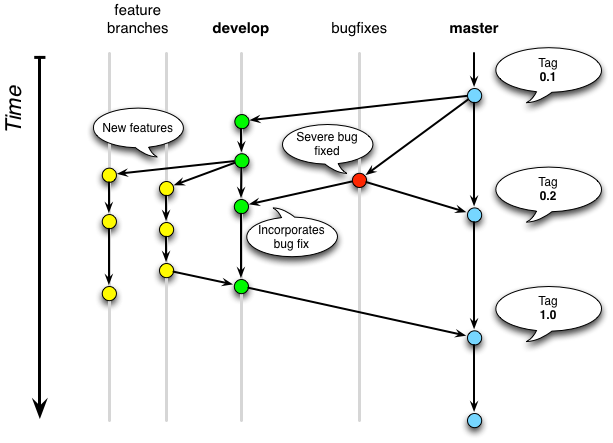
\includegraphics[height=\textheight]{images/git-workflow.png}
	% TODO: Bild abschneiden
\end{frame}

\begin{frame}{Best Practice}
	\begin{itemize}
		\item{Do commit early and often}
		\item{Do not panic (as long as you commited [or even added] your work)}
		\item{Do not change published history}
		\item{Do divide your work into different repositories}
		\item{Do useful commit messages}
		\item{Do keep up to date}
	\end{itemize}
\end{frame}

\section{Advanced Git Features}

\begin{frame}{}
  \begin{center}
    \huge\bfseries
    \textcolor{KITblack}{Advanced Git Operations}
  \end{center}
\end{frame}

% TODO 
% gitk
% git gui

% multiple remotes (pull workflow)

\begin{frame}{Stashing Your Work}
  \begin{itemize}
    \item Get rid of uncommitted changes temporarily
      \begin{shell}
        \$ git stash
      \end{shell}
    \item Resets your working copy to the last committed version $C$
    \item Creates a ``stash commit'' whose parent is $C$
    \item Puts the stash commit on a stack
    \item Top-most stash commit can be applied again using
      \begin{shell}
        \$ git stash pop
      \end{shell}
  \end{itemize}
\end{frame}
\begin{frame}{Rebase Your Branch on Other Branch}
  \begin{itemize}
    \item Most complex operation in git:
      \begin{shell}
        \$ git rebase origin/master
      \end{shell}
    \item Detach a commit from its parent and attach it to another commit
    \item Pre-condition is that changes can be applied to new parent
    \item Pro: Does not result in a merge-commit
    \item Contra: May create cascades of conflicts during rebase
  \end{itemize}
\end{frame}

\begin{frame}{Cherry-Picking}
  \begin{itemize}
    \item Take a commit from another branch and apply it to yours as well
      \begin{shell}
        \$ git cherry-pick <SHA>
      \end{shell}
    \item Pre-condition is that you did not change same lines
    \item Git keeps track of commits by SHA and can ignore double commits
  \end{itemize}
\end{frame}

\begin{frame}{Other Interesting Commands}
    \begin{shell}
      \$ git commit --amend \\
			\$ git add --patch/-p \\
			\$ git gui \\
			\$ git rebase -i \\
    \end{shell}
\end{frame}

%\section{Beyond Source Control}


\section{Appendix}

\begin{frame}{Further reads}
  \begin{columns}[T,onlytextwidth]
    \column{0.7\textwidth}
      \begin{itemize}
        \item \texttt{\$ man git} %\ldots\  just kidding
        \item Free Pro Git book at \url{http://git-scm.com/book}
        \item Different aspects from beginners to pros: \url{http://gitready.com}
        \item Git cheat sheet: \url{http://www.cheat-sheets.org/saved-copy/git-cheat-sheet.pdf}
				\item Interactive git tutorial: \url{https://try.github.io}
				\item Get these slides from: \url{http://github.com/ksetagit/kseta-dvcs-talk}\\
      \end{itemize}
    \column{0.3\textwidth}
      \centering
      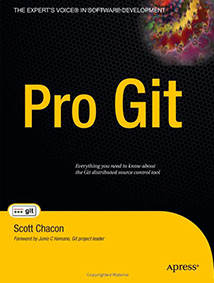
\includegraphics[width=1.5cm]{images/pro-git}
  \end{columns}
\end{frame}

\end{document}

% vim:sw=2
